%%%%%%%%%%%%%%%%%%%%%%%%%%%%%%%%%%%%%%%%%
% Report
% LaTeX Template
% Version 1.0 (December 8 2014)
%
% This template has been downloaded from:
% http://www.LaTeXTemplates.com
%
% Original author:
% Brandon Fryslie
% With extensive modifications by:
% Vel (vel@latextemplates.com)
%
% License:
% CC BY-NC-SA 3.0 (http://creativecommons.org/licenses/by-nc-sa/3.0/)
%
%%%%%%%%%%%%%%%%%%%%%%%%%%%%%%%%%%%%%%%%%

\documentclass[usletter, 12pt]{article}
%%%%%%%%%%%%%%%%%%%%%%%%%%%%%%%%%%%%%%%%%
% Contract Structural Definitions File Version 1.0 (December 8 2014)
%
% Created by: Vel (vel@latextemplates.com)
% 
% This file has been downloaded from: http://www.LaTeXTemplates.com
%
% License: CC BY-NC-SA 3.0 (http://creativecommons.org/licenses/by-nc-sa/3.0/)
%
%%%%%%%%%%%%%%%%%%%%%%%%%%%%%%%%%%%%%%%%%

\usepackage{geometry} % Required to modify the page layout
\usepackage{multicol}
\usepackage{amsmath}
\usepackage{amssymb}

\usepackage[pdftex]{graphicx}
\usepackage{wrapfig}
\usepackage[font=scriptsize, labelfont=bf]{caption}
\usepackage[utf8]{inputenc} % Required for including letters with accents
\usepackage[T1]{fontenc} % Use 8-bit encoding that has 256 glyphs

\usepackage{avant} % Use the Avantgarde font for headings
\usepackage{courier}
\usepackage{xparse}
\usepackage{xcolor}
\usepackage{listings}  % for code verbatim and console outputs

\setlength{\textwidth}{16cm} % Width of the text on the page
\setlength{\textheight}{23cm} % Height of the text on the page
\setlength{\oddsidemargin}{0cm} % Width of the margin - negative to move text left, positive to move it right
\setlength{\topmargin}{-1.25cm} % Reduce the top margin

\setlength{\parindent}{0mm} % Don't indent paragraphs
\setlength{\parskip}{2.5mm} % Whitespace between paragraphs
\renewcommand{\baselinestretch}{1.5}

\definecolor{green}{rgb}{0.18, 0.55, 0.34}

\graphicspath{ {figures/} }
\captionsetup[table]{skip=10pt}

\lstset{language=C, keywordstyle={\bfseries \color{black}}}

% defines algorithm counter for chapter-level
\newcounter{nalg}[section]

%defines appearance of the algorithm counter
\renewcommand{\thenalg}{\thesection .\arabic{nalg}}

% defines a new caption label as Algorithm x.y
\DeclareCaptionLabelFormat{algocaption}{Algorithm \thenalg}

% defines the algorithm listing environment
\lstnewenvironment{pseudocode}[1][] {
    \refstepcounter{nalg}  % increments algorithm number
    \captionsetup{font=normalsize, labelformat=algocaption, labelsep=colon}
    \lstset{
        breaklines=true,
        mathescape=true,
        numbers=left,
        numberstyle=\scriptsize,
        basicstyle=\footnotesize\ttfamily,
        keywordstyle=\color{black}\bfseries,
        keywords={input, output, return, parallel, function, for, to, in, if,
        else, foreach, while, and, or, new, print},
        xleftmargin=.04\textwidth,
        #1
    }
}{}

\renewcommand{\familydefault}{\sfdefault}  % default font for entire document
 % Input the structure.tex file which specifies the document layout and style

%----------------------------------------------------------------------------------------
%   DYNAMIC CONTRACT INFORMATION
%----------------------------------------------------------------------------------------

% Member's information
\newcommand{\project}{Project 1: Divide and Conquer}
\newcommand{\Sabbir}{Sabbir Ahmed}
\newcommand{\Zafar}{Zafar Mamarakhimov}

%----------------------------------------------------------------------------------------

\begin{document}

    %----------------------------------------------------------------------------------------
    %   TITLE PAGE
    %----------------------------------------------------------------------------------------

    \begin{titlepage}

        \vspace*{\fill} % Add whitespace above to center the title page content
        \begin{center}

            {\LARGE \project~Analysis Report}\\ [1.5cm]

            \today
            
            \vspace*{\fill}

            \Sabbir

            \Zafar

        \end{center}
        \vspace*{\fill} % Add whitespace below to center the title page content

    \end{titlepage}

    \section{Description}
    A recursive, divide-and-conquer algorithm was developed and analyzed to multiply together lists of complex numbers. Two different multiplication methods were used to compute the same products to analyze the crossover point.

        \subsection{Background}
        A complex number z is given by a real part x and an imaginary part y,
            \[ z=x+iy, \]
        where \textit{i} is the imaginary unit $\sqrt{-1}$.

        Multiplying two complex numbers are similar to multiplying polynomials. Let $z_{1}=x_{1}+iy_{1}$ and $z_{2}=x_{2}+iy_{2}$ be two complex numbers. Then their product is
            \[ z_{1}z_{2}=(x_{1}+iy_{1})(x_{2}+iy_{2})=(x_{1}x_{2}-y_{1}y_{2})+i(x_{1}y2+y_{1}x_{2}) \]

        That is, the real part of $z_{1}z_{2}$ is $x_{1}x_{2}-y_{1}y_{2}$ and the imaginary part is $x_{1}y_{2}+y_{1}x_{2}$. The computation of a single complex product requires four real products and two real additions (subtraction is just addition with one operand negative and the "+\textit{i}" doesn't count as an addition as this is really just notation to separate the real and imaginary parts).

        As it turns out, there is a way to reduce the number of real multiplications needed to compute a complex product. It is based on the following observation, which is similar to how Karatsuba's method for multiprecision multiplication was derived:
            \[ (x_{1}+y_{1})(x_{2}+y_{2})=x_{1}x_{2}+(x_{1}y_{2}+y_{1}x_{2})+y_{1}y_{2} \]

        Let $t$ denote the product $(x_{1}+y_{1})(x_{2}+y_{2})$; then if the real products $r=x_{1}x_{2}$ and $s=y_{1}y_{2}$ are computed, the complex product is just
            \[ z_{1}z_{2}=(r-s)+i(t-r-s) \]

        Now, this computation only requires three real multiplications, but increases the number of additions to five. Since multiplication is the more expensive operation, it is expected for the reduction in the number of multiplies to pay-off, at least if the numbers are large enough.

        Simply multiplying two complex numbers would not require a divide-and-conquer solution. However, to multiply a list of $n$ complex numbers, there is a natural recursive divide-and-conquer solution, which is to recursively multiply the left and right halves of the list, each of length approximately $\frac{n}{2}$, and then multiply together the results of the two recursive calls. The base case is a list of length one, for which the function simply returns the single value in the list.

        When multiplying a list of numbers, the difference between three or four real multiplications per complex multiplication can make a significant difference in the running time, especially if individual real multiplications are expensive. Multiprecision arithmetic is required to handle the growth of the product as the numbers get multiplied. Since the cost to perform a single real multiplication will increase per iteration, the use of the "three-multiply" complex multiplication is expected to be faster than the "four-multiply" version. However, since the three-multiply version requires more additions, it may not pay-off until the numbers are large or the list of numbers is long.

        The point at which the asymptotically better algorithm becomes faster is called the \textit{crossover point}.

    \section{Implementation}
    The project was written in C++11 and built with GCC v5.4.0. The GMP library, along with its C++ wrapper, GMPXX, was used to handle the multiprecision arithmetic. The recursive divide-and-conquer functions for both the three- and four-multiplication methods were implemented identical.

\begin{lstlisting}
/*
Uses a divide and conquer method to recursively multiply all the elements in
the complex array using either of the multiplication methods

Inputs:
    - complex_array (std::vector<mpz_class>):
        vector of GMP integer pairs
    - first, last (const size_t): first and last indices of the subarray

Outputs:
    - cmulx() outputs (std::vector<mpz_class>):
        final complex product
*/
std::vector<mpz_class> cmulx_list(
        std::vector<std::vector<mpz_class>> complex_array,
        const size_t first,
        const size_t last
) {

    // if length of the array is 1
    if (first == last) {
        return complex_array[first];
    }

    size_t mid = (first + last) / 2;

    return cmulx(
            cmulx_list(complex_array, first, mid),
            cmulx_list(complex_array, mid + 1, last)
    );

}
\end{lstlisting}

        % example of adding figures
        \iffalse
        \begin{figure}[ht]
            \begin{center}
                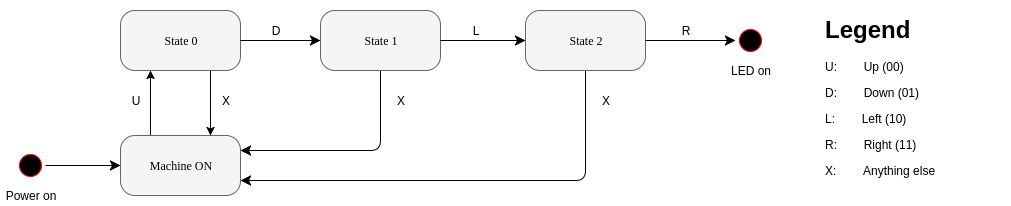
\includegraphics[width=1\textwidth]{figures/state_diagram.png}
                \caption{State Diagram Implementation of the Game with the Secret Code Mapped to 0b00011011} \label{fig:state_diagram}
            \end{center}
        \end{figure}
        \fi

    \section{Testing and Timing}
        \subsection{Testing Platform Specifications}

        Lorem ipsum dolor sit amet, consectetur adipisicing elit, sed do eiusmod
        tempor incididunt ut labore et dolore magna aliqua. Ut enim ad minim veniam,
        quis nostrud exercitation ullamco laboris nisi ut aliquip ex ea commodo
        consequat. Duis aute irure dolor in reprehenderit in voluptate velit esse
        cillum dolore eu fugiat nulla pariatur. Excepteur sint occaecat cupidatat non
        proident, sunt in culpa qui officia deserunt mollit anim id est laborum.

        % example of adding tables
        \iffalse
        \begin{table}[h]
            \caption{Example of values of registers after STATE1}
            \centering
            \begin{tabular*}{200pt}{@{\extracolsep{\fill}} c c c}

            \textbf{Register} & \textbf{Before} & \textbf{After} \\
            \hline
            USER & 0b01000000  & 0b01000000 \\
            CURSOR & 0b01000000 & 0b01000000  \\
            REALSTATE & 0b01000000 & 0b01000000 \\
            NSHIFT & 0b00000001 & 0b00000000 \\
            \hline
            \textbf{UART} & 1,D, & 1,D,D,2,S,\textbackslash n \\
            \end{tabular*}
        \end{table}
        \fi


\end{document}
